% LTeX: language=es-es
\chapter{Evaluación}

Para evaluar la solución se deben considerar dos aspectos de la implementación: el funcionamiento correcto del código en términos de entrada y salidas de datos en cada una de sus partes (unidades) y la consistencia del programa con las proyecciones de tiempo y espacio teóricos.


\section{\textit{Unit Testing}}

Para probar el funcionamiento del programa se utilizó la librería \textit{Catch2}\cite{catch2}, que permite fácilmente crear pruebas  unitarias (\textit{Unit Testing} en Inglés). Las unidades en este caso son las distintas clases creadas para representar las estructuras necesarias para el programa: \textit{\textbf{Permutation}} (véase \ref{lst:perm}: permutación con vectores de bits y atajos), \textit{\textbf{ARSSequence}} (véase \ref{lst:seq}: Secuencias utilizando permutaciones), \textit{\textbf{WaveletMatrix}} (véase \ref{lst:wlmt}: secuencia representada como matriz \textit{wavelet} utilizando vectores de bit), \textit{\textbf{Grid}} (véase \ref{lst:grid}: grilla utilizando matriz \textit{wavelet} y \textit{\textbf{PatternSearcher}} (véase \ref{lst:pattern}: buscador de patrones utilizando grilla y secuencia).

Como ejemplo, considérese la clase buscadora de patrones, se puede hacer pruebas que corroboren los resultados de la búsqueda:

\begin{lstlisting}[style=cppstyle, caption={\textit{\textit{Test }de búsqueda}}, label={lst:search-test}] 
TEST_CASE("PatternSearcher","[pattern]") {
    REQUIRE_FALSE(g_fileName.empty());
    string input_filename = g_fileName;
    FILE *input  = fopen(input_filename.c_str(), "rb");  
    string filecontent = "";
    char c;
    while (fread(&c, 1, 1, input) == 1) {
        filecontent += c;
    }
    fclose(input);
    PatternSearcher PS(input_filename);
    for (int i = 0; i < 50; i++) {
        string pattern = filecontent.substr(rand() % (filecontent.size() - 10), rand() % 10 + 1);
        cout << i << ": Searching for pattern: \"" << pattern << "\"" << endl;
        vector<int> occurences;
        PS.search(&occurences, pattern);
        sort(occurences.begin(), occurences.end());
        vector<int> expected_occurences = findOccurrences(filecontent, pattern);
        REQUIRE(occurences == expected_occurences);
    }    
}
vector<int> findOccurrences(const string& filecontent, 
    const string& pattern) {
    vector<int> occurrences;
    for (size_t i = 0; i < filecontent.size(); i++) {
        if (filecontent.substr(i, pattern.length()) == pattern) {
            occurrences.push_back(i);
        }
    }
    return occurrences;
}
\end{lstlisting}

La prueba mostrada cerciora que el método utilizado \textit{search} encuentre los índices de las ocurrencias del patrón generado aleatoriamente a partir del contenido del texto de entrada, comparándolos con los resultados arrojados por una función de búsqueda sobre el contendido (visto como un \textit{string}) que utiliza funciones estándar en C++ para encontrar, en tiempo $\mathcal{O}$(\textit{n}), las ocurrencias.

\section{Análisis empírico}
\subsection{Espacio}

El espacio total de la estructura corresponde a la suma de los valores del espacio de la grilla \textit{G}, el espacio de la secuencia \textit{R}, el espacio de la secuencia \textit{l}, los vectores que mapean los símbolos normalizados a los originales y el símbolo inicial:
\[
SPACE(PS) = 32 + r \log n + 2 \times 8 \times 256  + SPACE(G) + SPACE(R)
\]

El espacio de la grilla \textit{G} es igual al espacio de la matriz \textit{wavelet} \textit{WM} y los valores para guardar la cantidad de columnas, filas y puntos:
\[
SPACE(G) = 3 \times 32 + SPACE(WM)
\]

El espacio de la matriz \textit{wavelet} \textit{WM} corresponde al valor de $\sigma$, el vector de $z_l$ de largo $\log \sigma$ y el vector de largo $\log \sigma$ de vectores de bits de largo \textit{n}. En este caso, como la matriz se construye sobre la secuencia formada por los índices de las reglas, $\sigma$ y \textit{n} son ambos la cantidad de reglas:
\[
SPACE(WM) = 32 + 32 \log r + SIZE(BV) \log r 
\]

El vector de bits tiene, en el peor caso, un tamaño de $1.5n$, con lo que el tamaño total de la matriz queda:
\[
SPACE(WM) = 32 + 32 \log r +1.5 r \log r 
\]

Con esto, el espacio de la grilla G queda:
\[
SPACE(G) = 3 \times 32 + 32 + 32 \log r + 1.5 r \log r 
\]
\[
SPACE(G) = 96 + 32 \log r + 1.5 r \log r 
\]

El espacio usado por una secuencia \textit{R} de largo \textit{n} sobre un alfabeto $\sigma$ representada por permutaciones es igual a la suma de los $A_i$ y $D_i$ que hacen un total de $4n + o(n)$ más las permutaciones que usan un espacio total de $n \log \sigma + n o(\log \sigma)$. Como \textit{R} se construye sobre la secuencia de largo 2\textit{r} y el alfabeto corresponde a la suma del alfabeto del texto $\sigma$ y la cantidad de reglas \textit{r}, sobrestimando los ordenes \textit{o} queda el espacio como:
\[
SPACE(R) = 10r + 2 r \log {(r + \sigma)}
\]

El espacio total en bits de la estructura es entonces:
\begin{equation}
    SPACE(PS) = 4224 + r \log n +  + 32 \log r + 1.5 r \log r + 10r + 2 r \log {(r + \sigma)} \label{eq:space}
\end{equation}
\iffalse
Si se analiza esta expresión para que cumpla ser menor que el tamaño del texto $8n$ y comprimir efectivamente el texto, considérese para un \textit{n} suficientemente largo como negligentes los valores 4224 y $\sigma$, entonces se tiene la inecuación: 
\[
r\log n + 32\log r + 3.5r\log r + 10 r < 8n
\]

Si se asume $r = n ^ x$
\[
n^{x} \log n + 32\log n^{x} + 3.5n^{x}\log n^{x} + 10 n^{x} < 8n
\]
Se necesita entonces que cada uno de estos términos crezca de manera sub-lineal. Si se toma $x = 1$, $n^{x} \log n$ y $10 n^{x}$ crecen muy rápido. Probando entonces con $x = \frac{1}{2}$:
\[
n^{\frac{1}{2}} \log n + 32\log n^{\frac{1}{2}} + 3.5n^{\frac{1}{2}}\log n^{\frac{1}{2}} + 10 n^{\frac{1}{2}} < 8n
\]
Cada uno de los términos crece de manera sub-lineal y por lo tanto el texto es comprimido con un \textit{r} equivalente a $\sqrt{n}$ o menos.
\fi

\newpage
\subsubsection{Construcción}
\label{sect:construct-space}

El proceso de construcción de la estructura, según los propuesto en el libro, utiliza extras $\mathcal{O}(c + n)$ bits. En la implementación, el tamaño extra usado aparece en el proceso de construcción de la matriz:
\begin{lstlisting}[style=cppstyle, caption={Construccion de matriz}, label={lst:wm-build}] 
void WaveletMatrix::build(vector<u32>& S, u32 n, u32 sigma) {
    vector<u32> S_hat(n);
    bit_vector M(n, 0);
    bit_vector M_hat(n, 0);
    u32 m = sigma;
    for (u32 l = 0; l <= ceil(log2(sigma))-1; l++) {    
        u32 z_l = 0;
        bit_vector B_l(n, 0);
        for (u32 i = 0; i < n; i++) {
            if (S[i] <= (m - M[i] + 1) / 2) { 
                B_l[i] = 0;
                z_l++;
            } else {
                B_l[i] = 1;
                S[i] = S[i] - (m - M[i] + 1) / 2;
            }
        }
        bm.push_back(ppbv(B_l));
        z.push_back(z_l);
        if (l < ceil(log2(sigma)) - 1) {
            u32 p_l = -1; // max value + 1 = 0
            u32 p_r = z[l] - 1;
            u32 p;
            int n_ = n;
            for (u32 i = 0; i < n_; i++) {
                u32 b = bm[l][i];
                if (b == 0) {                    
                    p_l ++;  
                    p = p_l;
                } else {                    
                    p_r ++;
                    p = p_r;              
                }
                S_hat[p] = S[i];
                if (m % 2 == b) {
                    M_hat[p] = b;
                } else {
                    M_hat[p] = M[i];
                }
                if ((m+1)/2==2 && M_hat[p] == 1) {
                    n = n-1;;
                }
            }        
            swap(S, S_hat);
            swap(M, M_hat);
            m = (m+1)/2;
        }
    }
    S.clear();
    S.shrink_to_fit();
}
\end{lstlisting}
Esto ocupa, efectivamente, $2 n$ bits para los vectores de bit y $\mathcal{O}(n)$ bits para la secuencia auxiliar, lo que indica que la implementación es consistente con lo esperado según el análisis.

Si se utiliza memoización para expandir las reglas al momento de comparar y ordenar la secuencia, se requiere, en el peor caso, $\mathcal{O}(2n)$ \textbf{bytes} (¡no bits!) de memoria extra, considerando un árbol sintáctico binario balanceado de \textit{n} nodos. Incluso en el mejor caso, la memoria de la memoización requiere al menos \textit{n} bytes. Es posible mejorar esto guardando las expansiones de las reglas que más se repiten en el árbol (por ejemplo, las que otrora apareciesen en la secuencia \textit{C} generada por \textit{Re-Pair}), y memoizar sólo prefijos de las reglas de cierto tamaño. En este caso es quizás posible utilizar otras estructuras como un \textit{trie} o un \textit{suffix-tree} en vez del mapa \textit{int} a \textit{string} utilizado como memoria.

\subsection{Tiempo}

\subsubsection{Construcción}

En teoría, la construcción de una estructura grilla usando matrices \textit{wavelet} con \textit{n} puntos y \textit{c} columnas demora tiempo $\mathcal{O}(c + n \log{n})$\cite[Capítulo 10.6]{Navarro}. Esto se debe a que primero se deben ordenar los puntos por la coordenada \textit{x}, y luego se recorren estos para inicializar los vectores de bits. 

En el caso particular de la búsqueda de patrones, no es necesario ordenar los puntos. En efecto, la clase buscadora primero ejecuta \textit{Re-Pair} sobre el texto de largo \textit{n} (tiempo $\mathcal{O}(n)$), después la normalización (tiempo $\mathcal{O}(n)$), para luego ordenar la secuencia \textit{R} de reglas por orden lexicográfico de la expansión reversa del lado izquierdo ($\mathcal{O}(r \log r)$ comparaciones donde expandir toma, en promedio, $\mathcal{O}(\log n)$). Los puntos son entonces creados de forma que las columnas estén ordenadas por el valor lexicográfico del lado derecho (tiempo $\mathcal{O}(r \log r \log n)$). 

Todo lo anterior significa que la grilla entonces toma tiempo $\mathcal{O}(r)$, que sumado al tiempo necesario para ordenar la secuencia \textit{R}, conlleva a un tiempo total de:

\begin{equation}
\mathcal{O}(n + r \log r \log n)
\label{eq:theo}
\end{equation}

Con \textit{n} el largo del texto y \textit{r} la cantidad de reglas.

Se pudo medir el tiempo de construcción de la implementación utilizando textos reales, obtenidos del sitio \textit{Project Gutenberg}\cite{guthenberg}. Para cada texto, se ejecutó la construcción de la clase buscadora de patrones varias veces, y se obtuvo el promedio de todas estas medidas. Los resultados se pueden ver en la figura \ref{fig:timecst}, donde se comparan con la predicción teórica calculada \ref{eq:theo}.

\begin{figure}[h!]
    \centering
    \captionsetup{position=above} % Places the caption above the image
    \caption{Tiempo de construcción de la estructura en función del número de reglas, comparado a tiempo teórico $\mathcal{O}(n + r \log{r} \log {n})$}
    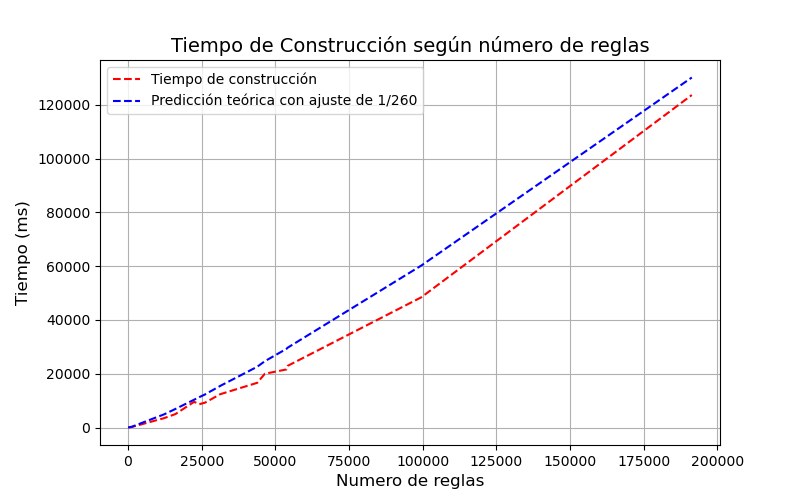
\includegraphics[width=1\textwidth]{imagenes/Time_Construction.png} % Adjust width as needed
    \label{fig:timecst}
\end{figure}

La implementación demuestra comportarse exactamente como lo predicho por la fórmula obtenida del análisis teórico.

ES posible, con memoización, reducir el tiempo de construcción significativamente. Como las primeras reglas corresponden a las reglas creadas por \textit{Re-Pair}, estas se expanden primero y se guardan. Luego, el resto de las reglas corresponden a las reglas extras creadas para reducir la secuencia \textit{C}, y por lo tanto utilizan todas la memoización de forma consecutiva. Sin embargo, esta técnica utiliza significativa memora extra, y no logra comprimir el texto. 



\subsubsection{Búsqueda}


El costo de tiempo teórico para reportar \textit{occ} ocurrencias de un patrón \textit{P} de largo \textit{m} en el texto \textit{T} de largo \textit{n} es:
\[
\mathcal{O}( (m + \log{n}) m \log{r} \log{\log{r}} + \textit{occ} \log{n} \log{\log{r}}  )
\]

Esto se debe a que en una gramática balanceada, el árbol sintáctico tiene altura $\log{n}$, y la operación de acceso en la secuencia representada por permutaciones (\textit{R}) tiene un tiempo $\mathcal{O}(\log \log r)$. De aquí que el primer sumando en la expresión teórica corresponde a expandir \textit{m} símbolos de una regla ($(m + \log{n}) \log{\log{r}}$), por cada comparación en la búsqueda binaria ($\log{r}$), por cada división de sufijo y prefijo del patrón (\textit{m}). El segundo sumando en tanto corresponde a recorrer virtualmente hasta la raíz el árbol sintáctico ($\log{n}$), por cada ocurrencia encontrada (\textit{occ}), haciendo accesos en \textit{R} ($\log{\log{r}}$).

Para medir el tiempo de búsqueda de la implementación en función de los parámetros, se crearon textos que permitiesen mantener fijos algunos de estos y variar el parámetro relevante. Por ejemplo, dado un texto $T = (a^{i}b)^j$ con $i \geq 0$ y $j > 0$, las búsquedas para cualquier patrón $P = a^{k}b$ con $0 \leq k \leq i$ reportan siempre \textit{j} ocurrencias. Con esto se puede medir como varía el tiempo en función del largo de \textit{P}. La figura \ref{fig:timepl} muestra las mediciones de tiempo para la búsqueda de un patrón $a^{k}b \backslash n$ en el texto donde ese patrón entrega la misma cantidad de ocurrencias, independiente del valor de \textit{k}.

\begin{figure}[h!]
    \centering
    \captionsetup{position=above} % Places the caption above the image
    \caption{Tiempo de búsqueda en función del largo del patrón para un mismo número de ocurrencias}
    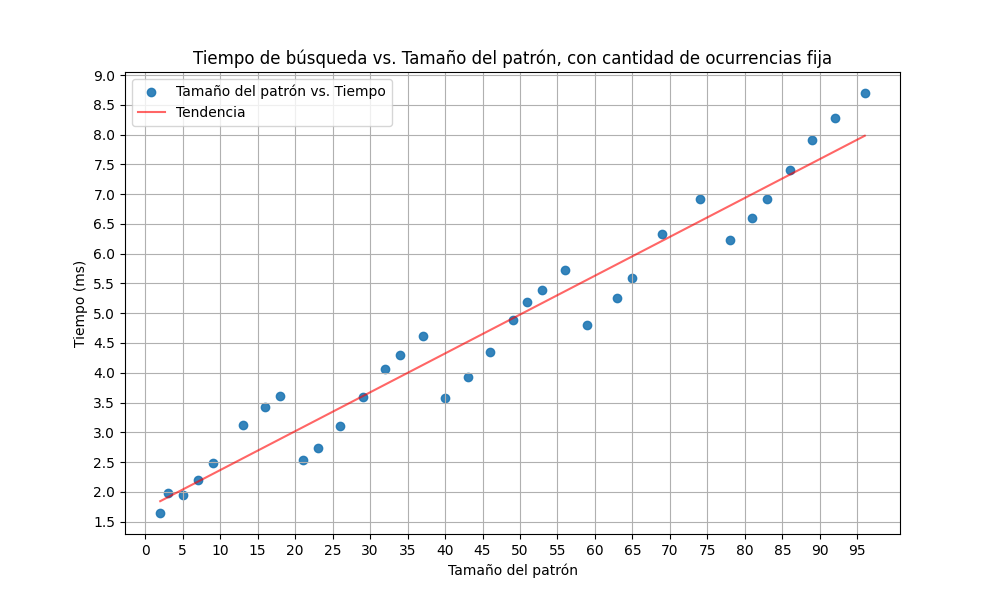
\includegraphics[width=1\textwidth]{imagenes/TIME_FIXED_OCC.png} % Adjust width as needed
    \label{fig:timepl}
\end{figure}

La implementación demuestra un rendimiento equivalente al análisis teórico de la función de búsqueda.

El tiempo en función de la cantidad de ocurrencias requiere mantener fijo el largo de los patrones de búsqueda (además de los otros parámetros). Una solución simple fue usar los bigramas (secuencias de largo 2) más comunes en Inglés\cite{bigram} como los patrones a buscar. Luego se buscan las ocurrencias de estos patrones en varios textos en inglés. Los gráfico de estas medición para cada texto real utilizado correspondes a la figuras de la tablas \ref{tab:searches} y \ref{tab:searchescont}. El gráfico \ref{fig:timeoccs} muestra la combinación de todas las mediciones y la tendencia combinada polinomial de primer grado. 

La figura \ref{fig:timeoccsprediction} ilustra el tiempo teórico para fines de cerciorar el mismo crecimiento, utilizando valores promedios de \textit{n} y \textit{r}. La justificación para esto es que, aunque el tiempo de búsqueda es función de \textit{n} y \textit{r}, además de \textit{occ}, es posible un análisis más simple considerando \textit{r} y \textit{n} como funciones lineales de \textit{occ} en textos reales, donde independiente del largo el texto no se vuelve menos o más predictivo, y la "densidad" de ocurrencias se mantiene igual. 

\begin{figure}[h!]
    \centering
    \captionsetup{position=above} % Places the caption above the image
    \caption{Tiempo de búsqueda en función del número de ocurrencias para un patrón de largo dos}
    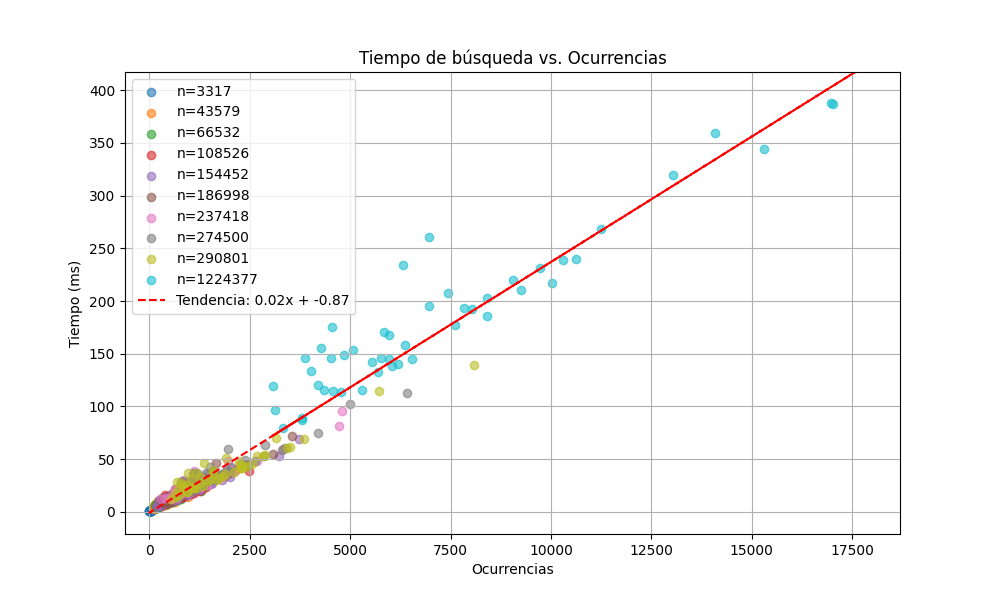
\includegraphics[width=1\textwidth]{imagenes/Time_Fixed_Pattern.png} % Adjust width as needed
    \label{fig:timeoccs}
\end{figure}

\begin{figure}[h!]
    \centering
    \captionsetup{position=above} % Places the caption above the image
    \caption{Tiempo de búsqueda en función del número de ocurrencias para un patrón de largo dos con predicción teórica usando promedio de \textit{n} y \textit{r}, con tiempo teórico 
    $ O( (m + \log{n}) m \log{r} \log {\log {r}} + occ \log{n} \log {r} ) $.}
    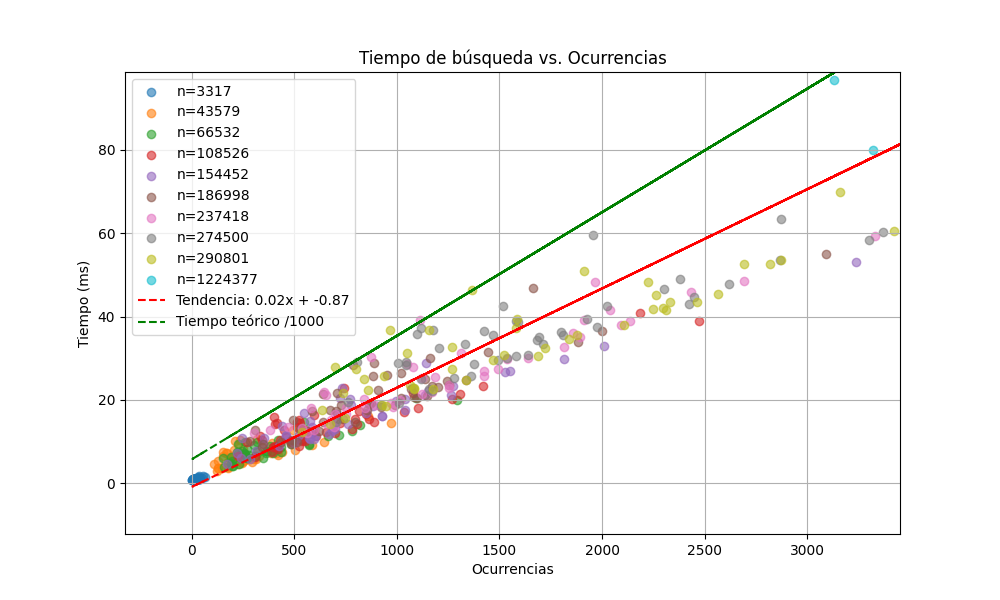
\includegraphics[width=1\textwidth]{imagenes/TIME_SEARCH_ZOOM.png} % Adjust width as needed
    \label{fig:timeoccsprediction}
\end{figure}

\begin{figure}[]
    \centering
    \captionsetup{position=above}
    \caption{Tiempos de búsquedas en \textit{ms} (milisegundos) en función del número de ocurrencias para un patrón de largo 2}
    \hspace*{-\marginparwidth}
    \begin{tabular}{cc} % Two columns      
        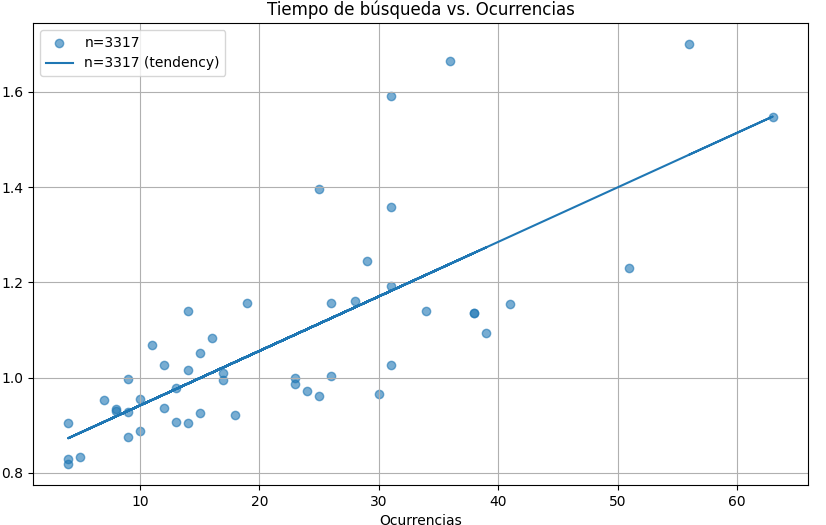
\includegraphics[width=0.55\textwidth]{imagenes/Figure_3317.png} & 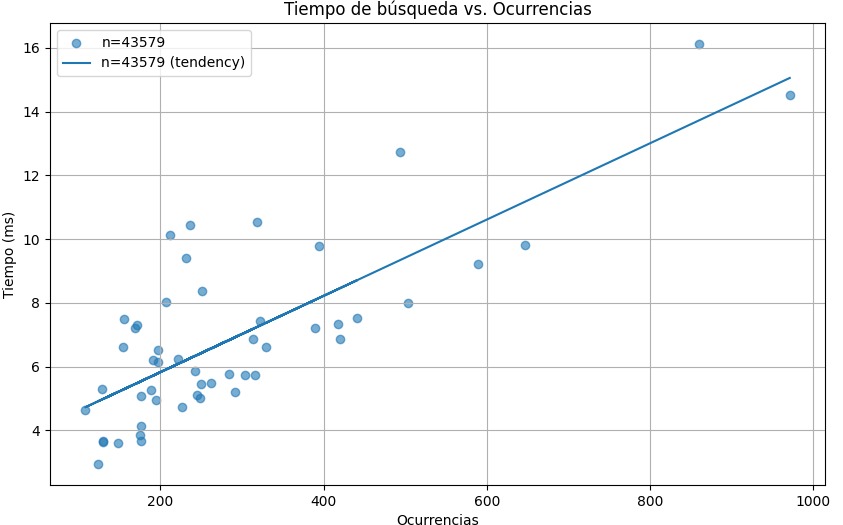
\includegraphics[width=0.55\textwidth]{imagenes/Figure_43579.png} \\
        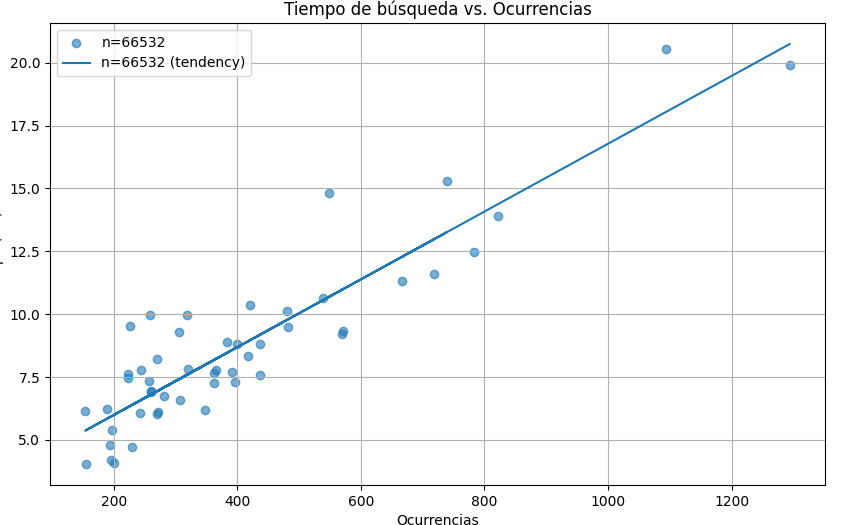
\includegraphics[width=0.55\textwidth]{imagenes/Figure_66532.png} & 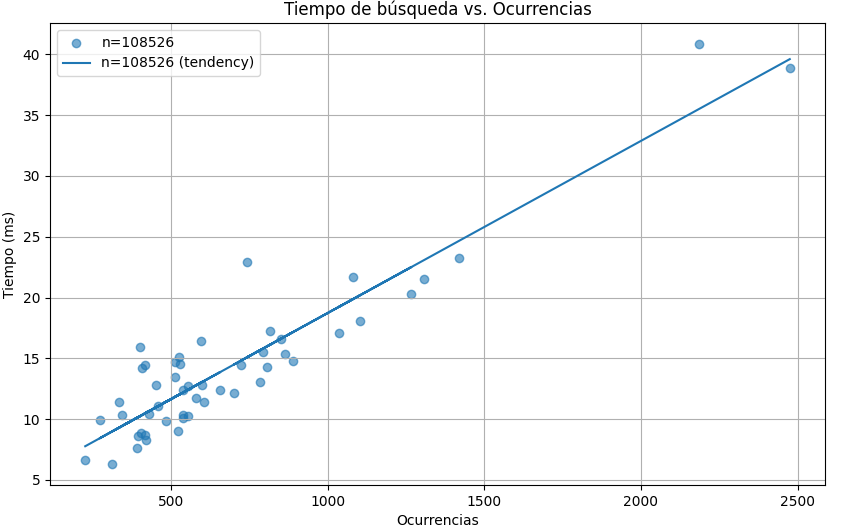
\includegraphics[width=0.55\textwidth]{imagenes/Figure_108526.png} \\
        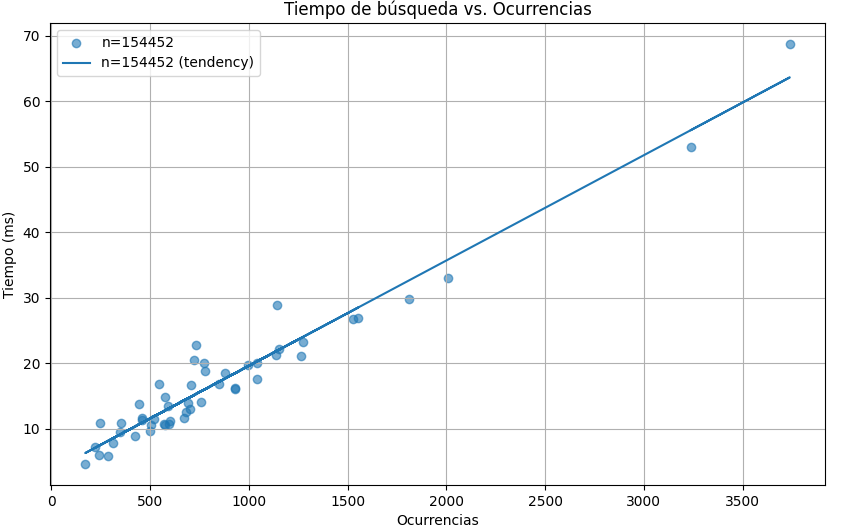
\includegraphics[width=0.55\textwidth]{imagenes/Figure_154452.png} & 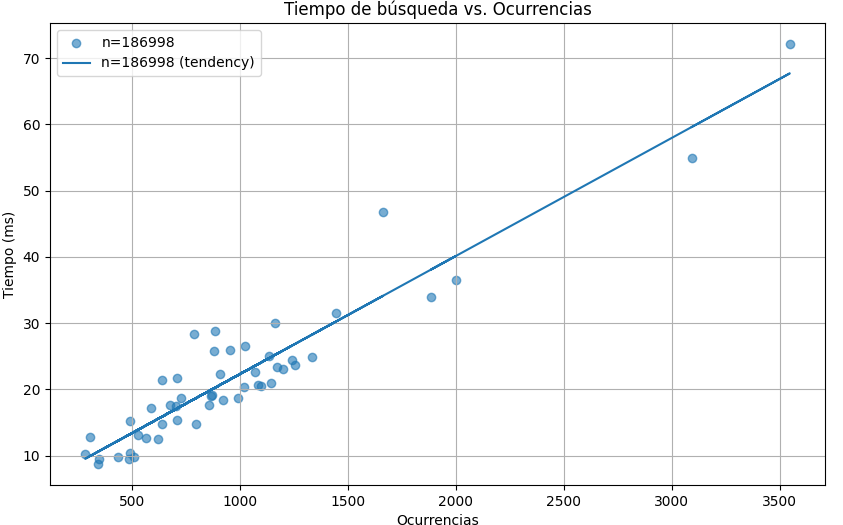
\includegraphics[width=0.55\textwidth]{imagenes/Figure_186998.png} \\
        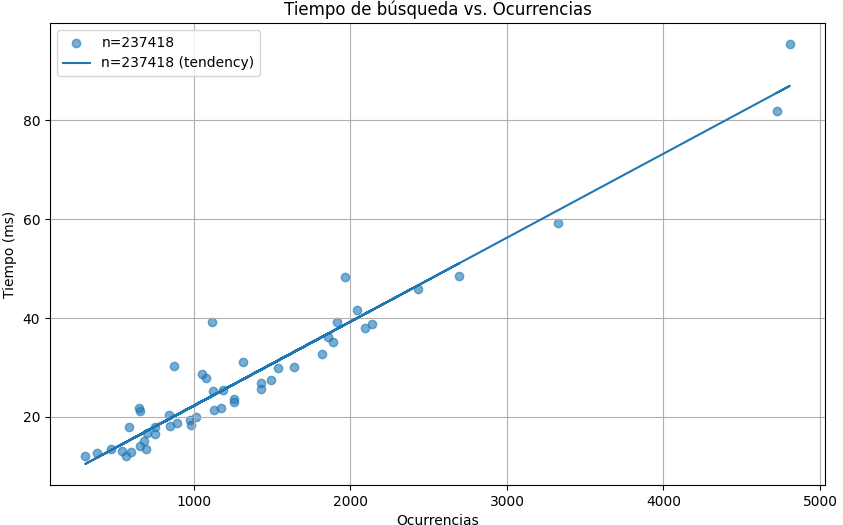
\includegraphics[width=0.55\textwidth]{imagenes/Figure_237418.png} & 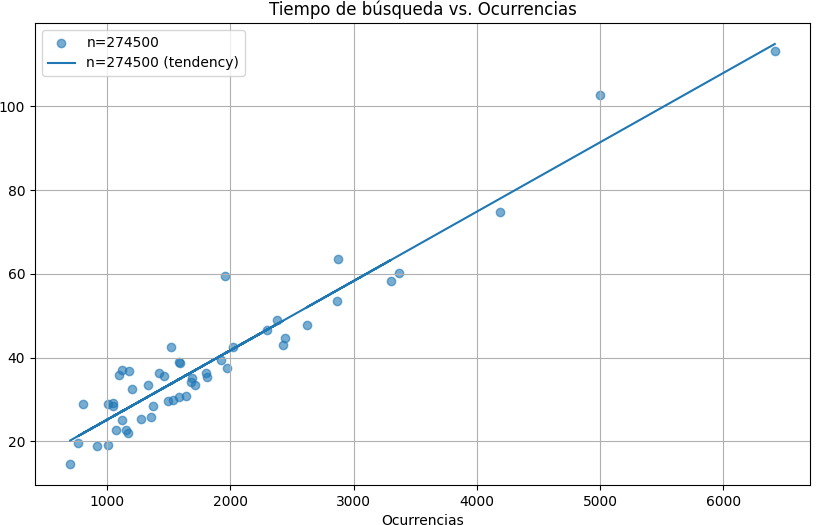
\includegraphics[width=0.55\textwidth]{imagenes/Figure_274500.png} \\
    \end{tabular}    
    \label{tab:searches}
\end{figure}

\begin{figure}[]
    \centering
    \captionsetup{position=above}
    \caption{Tiempos de búsquedas en \textit{ms} (milisegundos) en función del número de ocurrencias para un patrón de largo 2 (Continuación)}
    \hspace*{-\marginparwidth}
    \begin{tabular}{cc} % Two columns      
        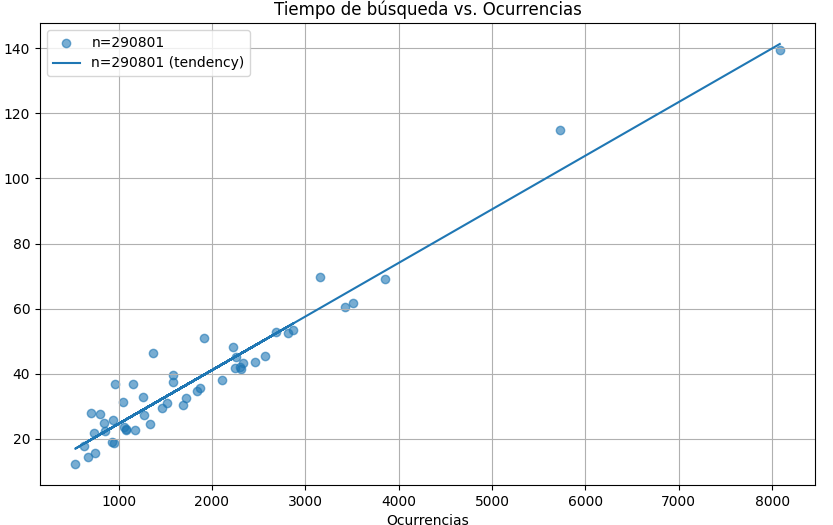
\includegraphics[width=0.55\textwidth]{imagenes/Figure_290801.png} & 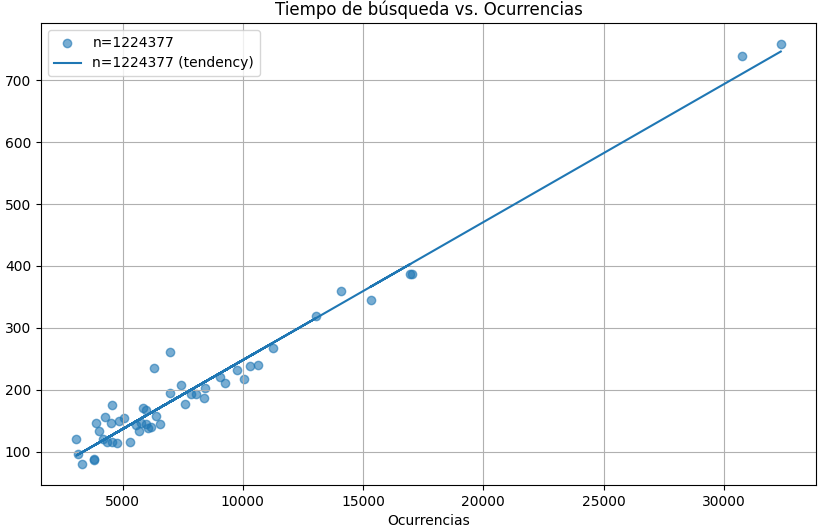
\includegraphics[width=0.55\textwidth]{imagenes/Figure_1224377.png} \\
    \end{tabular}    
    \label{tab:searchescont}
\end{figure}



El tiempo de búsqueda corresponde a la suma de los tiempos de búsqueda binaria de rangos en la grilla, el costo temporal de reportar las reglas dentro de estos rangos y los tiempos de búsqueda de ocurrencias para cada regla reportada. 

La búsqueda binaria demora en el peor caso $m\log{c}$, pues la comparación puede requerir expandir la regla entera hasta el largo del patrón (\textit{m}), y la regla puede corresponder a la regla inicial que expande al texto inicial de largo \textit{n}. En la práctica, con un texto real, la gran mayoría de las comparaciones terminan en el primer símbolo de la expansión. Esto es fácil de ver: como la distribución de los primeros símbolos de las expansiones de las reglas es aproximadamente uniforme (en realidad, es la distribución según las frecuencias de los símbolos en el lenguaje específico) las comparaciones perezosas retornarán falso en el primer símbolo. 

En un texto altamente repetitivo, las expansiones serán más largas, sin embargo, la cantidad de reglas es mucho menor que la de un texto real. Esto significa que no sólo la búsqueda binaria se hace sobre un espacio menor, el reporte de ocurrencias se hace sobre un árbol más corto (si se considera la búsqueda de ocurrencias como el recorrido del árbol sintáctico hasta la raíz).

Las pruebas de medición de tiempo muestran resultados consistentes a lo esperado en todos los casos, por lo cual se puede concluir que la implementación es correcta. 

\newpage
\section{Análisis en textos altamente repetitivos}
\label{sect:repet}

Las colecciones de textos reales altamente repetitivos de \textit{Pizza \& Chili Corpus}\cite{pizzachili_repcorpus} sirven como entradas para pruebas del mismo tipo a las utilizadas por el índice comprimido basado en gramática\cite{claude2020} y son por lo tanto una buena forma de analizar la competitividad de la estructura utilizada. El tamaño de los textos varía desde 45 MiB (\textit{world\_leaders}) a 446 MiB (\textit{einstein.en}), con variados grados de repetición, como se ve en la tabla \ref{tab:collect}. En la misma tabla aparece el espacio de la estructura para cada set de datos como \textbf{\textit{bps}} (bits por símbolo). 

\iffalse
\begin{table}[h!]
\centering
\begin{tabular}{|l|c|c|c|c|}
\hline
\textbf{Colección} & \textbf{Largo} & \textbf{Reglas} & \textit{bps} (estimación) & \textit{bps} (real) \\ \hline  
world\_leaders & 46968181 & 307066 &  0.649 & 8.224 \\ \hline  
Escherichia\_Coli & 112689515 & 3619577 &  3.629 & 40.560\\ \hline  
influenza & 154808555 &1557878 &  1.098 & 12.757 \\ \hline  
kernel & 257961616 &1129349 &  0.474 & 5.532 \\ \hline  
coreutils & 205281778 & 1994376 & 1.077 & 12.270\\ \hline
para&429265758 &4222046 &  1.138 & 12.463 \\ \hline  
cere & 461286644 & 3212008 & 0.796 & 8.809 \\ \hline
einstein.en & 467626544  & 163417 &  0.034 & 0.441 \\ \hline  
\end{tabular}
\caption{Propiedades de cada colección}
\label{tab:collect-old}
\end{table}
Nótese que la medida real de \textit{bps} es mucho más alta que la estimada y eso se debe a la forma en que están implementados los vectores de bits de la librería \textit{SDSL}\cite{sdsl-lite}: estos vectores de bits que corresponden a los pedazos de la secuencia representada por permutaciones no son buenos para tamaños muy pequeños, ya que la cantidad de memoria usada por los metadatos de la implementación del vector son del orden de los 136 Bytes (1088 bits). Por consiguiente, teniendo en cuenta que estos vectores se crean en proporción al alfabeto de tamaño \textit{r}, y la gran mayoría de estos vectores de bits tienen largo 2 bits (de hecho, todos los que corresponden a las reglas extras generadas en \ref{sect:extrar}), sumado a esto la misma magnitud de bits para soportar \textit{rank} y \textit{select}, el tamaño total empírico de los vectores en la secuencia representada por permutaciones es ordenes mayores a lo estimado (para las colecciones medidas, los \textit{bps} reales son 10 veces más grande a los esperado). Una solución a este problema se discute en la sección \ref{section:medic}.
\fi

\begin{table}[h!]
\centering
\begin{tabular}{|l|c|c|c|c|}
\hline
\textbf{Colección} & \textbf{Largo} & \textbf{Reglas} & \textit{bps}\\ \hline  
world\_leaders & 46968181 & 307066 &  0.848511 \\ \hline  
Escherichia\_Coli & 112689515 & 3619577 &  4.55733 \\ \hline  
influenza & 154808555 &1557878 & 1.40496\\ \hline  
kernel & 257961616 &1129349 & 0.619162 \\ \hline  
coreutils & 205281778 & 1994376 & 1.36035 \\ \hline
para&429265758 &4222046 &  1.41742 \\ \hline  
cere & 461286644 & 3212008 & 0.986939 \\ \hline
einstein.en & 467626544  & 163417 &  0.0475765 \\ \hline  
\end{tabular}
\caption{Propiedades de cada colección}
\label{tab:collect}
\end{table}



Para cada colección se hicieron búsquedas de patrones aleatorios de ciertos largos y se midieron los tiempos de búsqueda por ocurrencia. La figura \ref{fig:searchpizza} muestra los resultados obtenidos, ilustrados en un gráfico donde las escalas de ambos ejes son logarítmicas, y el eje \textit{Y} corresponde a los tiempos por ocurrencia (en teoría, $\mathcal{O}( (m + \log{n}) m \log{r} \log{\log{r}} + \textit{occ} \log{n} \log{\log{r}}) / \textit{occ}$), mientras que el eje \textit{X} corresponde a la cantidad \textit{occ} de ocurrencias detectadas.  

\begin{figure}
    \centering
    \captionsetup{position=above}
    \caption{Tiempos por ocurrencia en $\mu s$ (microsegundos) de búsquedas en función del número de ocurrencias para distintas colecciones repetitivas. Ambos ejes están es escala logarítmica}
    \hspace*{-\marginparwidth}
    \begin{tabular}{cc} % Two columns      
        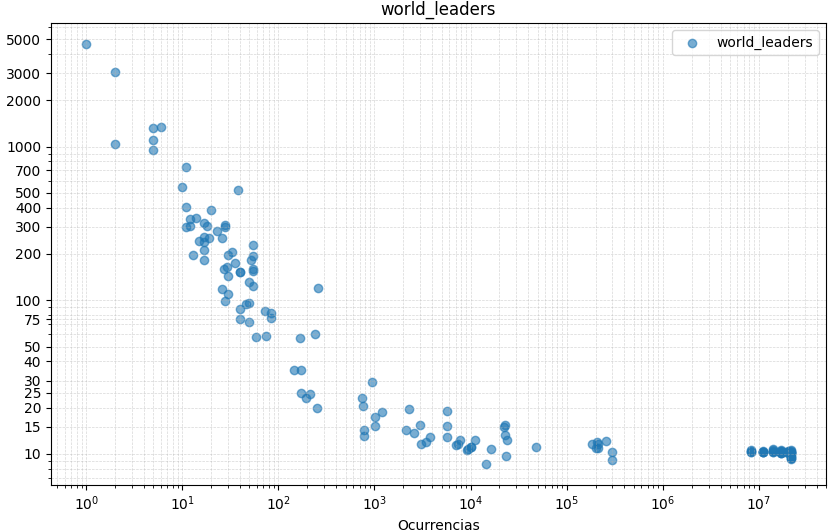
\includegraphics[width=0.55\textwidth]{imagenes/SEARCH_world_leaders.png} & 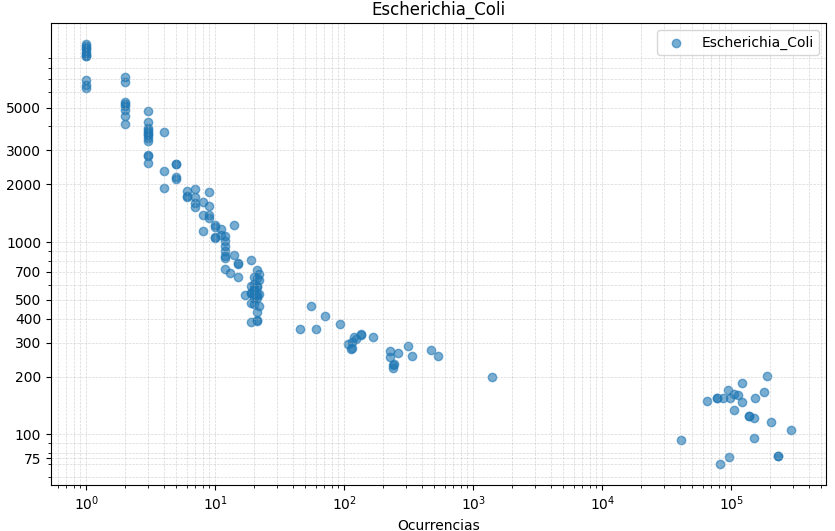
\includegraphics[width=0.55\textwidth]{imagenes/SEARCH_Escherichia.png} \\
        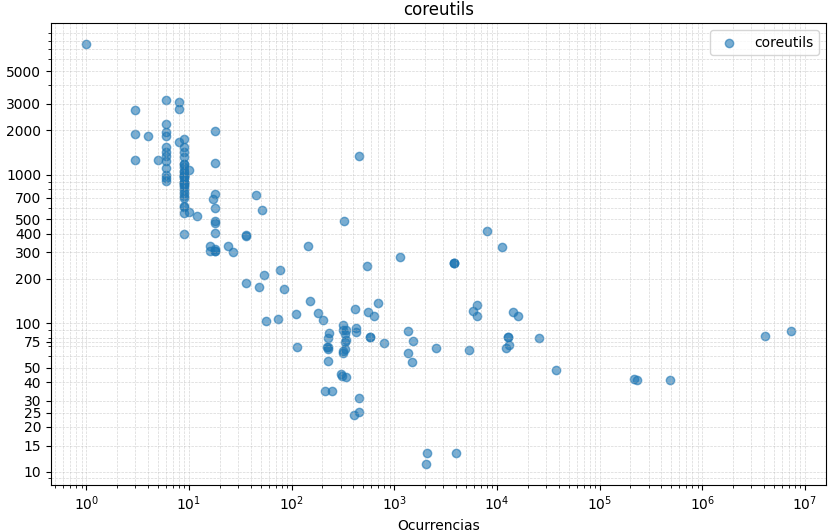
\includegraphics[width=0.55\textwidth]{imagenes/SEARCH_coreutils.png} & 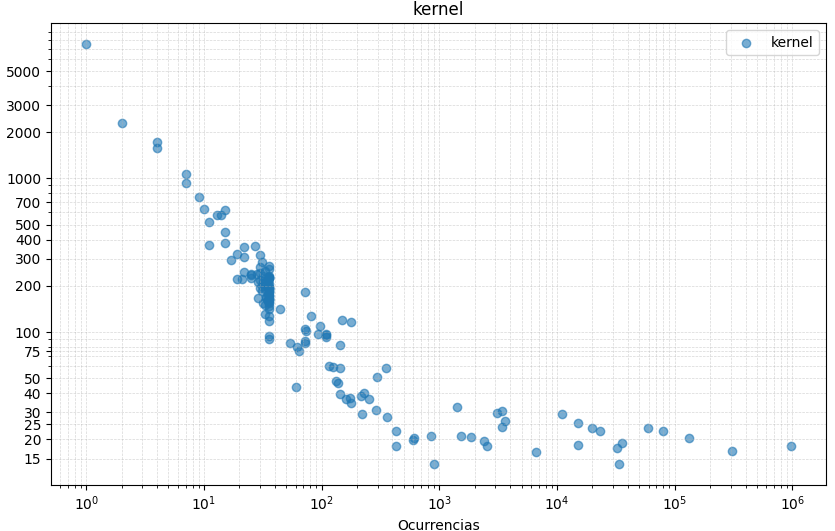
\includegraphics[width=0.55\textwidth]{imagenes/SEARCH_kernel.png} \\
        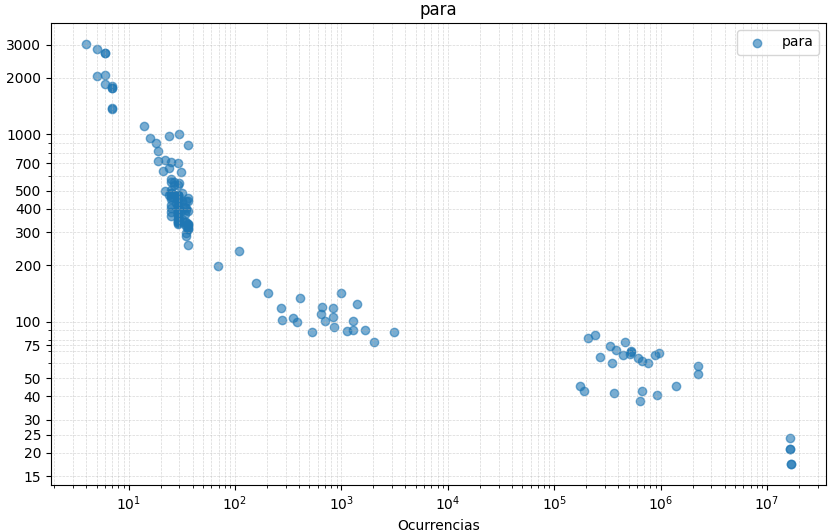
\includegraphics[width=0.55\textwidth]{imagenes/SEARCH_para.png} & 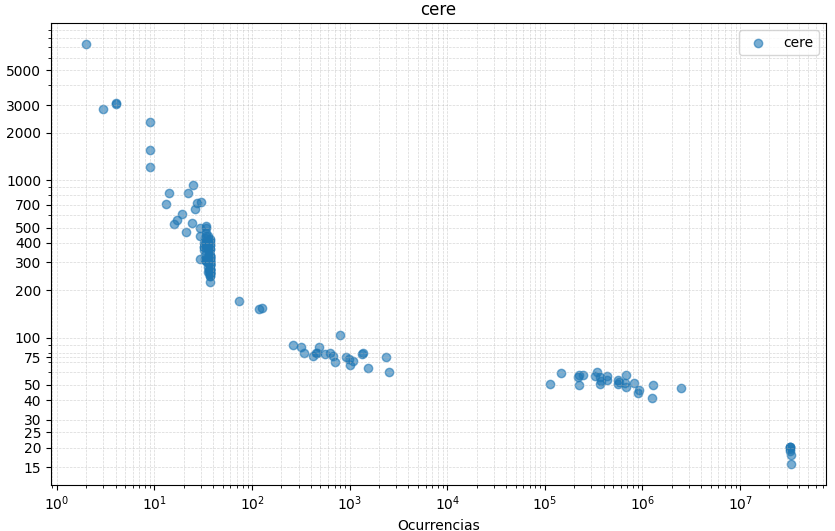
\includegraphics[width=0.55\textwidth]{imagenes/SEARCH_cere.png} \\
        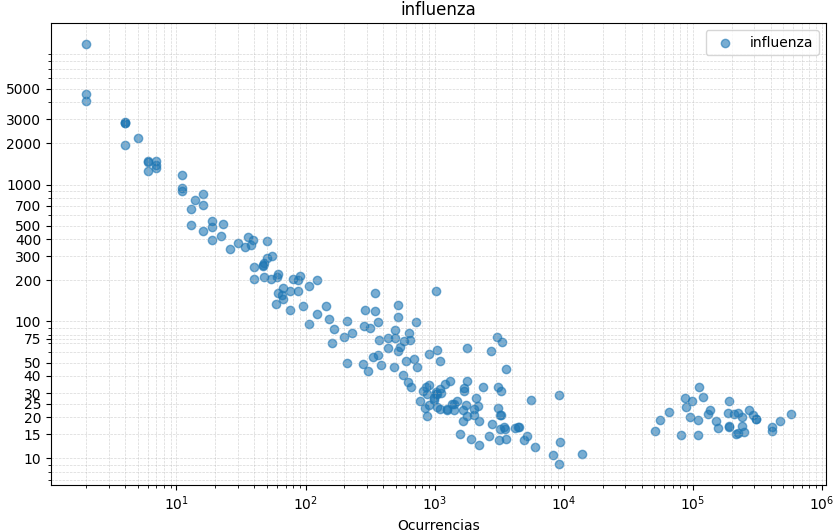
\includegraphics[width=0.55\textwidth]{imagenes/SEARCH_influenza.png} & 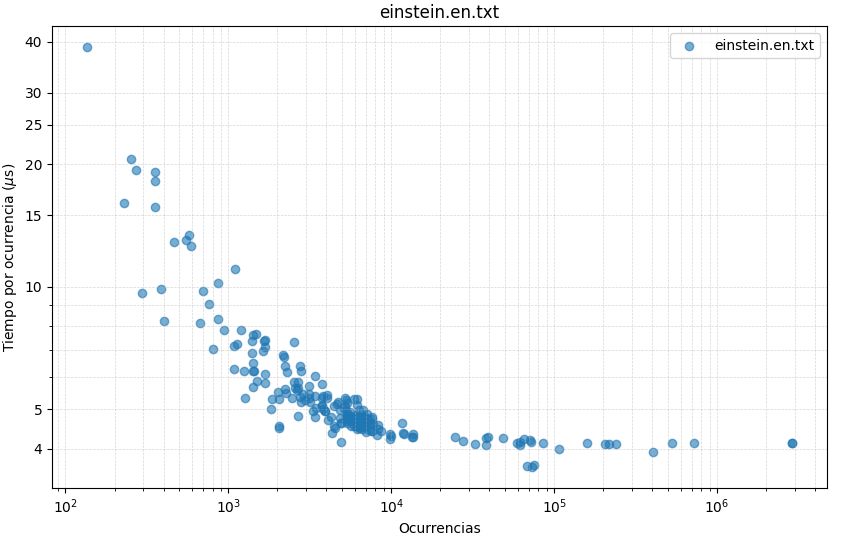
\includegraphics[width=0.55\textwidth]{imagenes/SEARCH_einstein.png} \\
    \end{tabular}    
    \label{fig:searchpizza}
\end{figure}

La estructura toma tiempos menores por ocurrencia mientras más ocurrencias del patrón se encuentren en el texto. Patrones de menos largo aparecen con más incidencia en los textos y por lo tanto el proceso de dividir el patrón en todos sus posible sufijos y prefijos es más corto. 

En colecciones altamente repetitivas como \textit{einstein.en} logra tiempos de búsqueda por ocurrencia bajo 5 $\mu s$ cuando la cantidad de ocurrencias es del orden de $10^4$ o mayor. En \textit{world\_leaders} el tiempo por ocurrencia se estabiliza en 9 a 10 $\mu s$. En otras colecciones el tiempo por ocurrencia es menos estable: en \textit{influenza} altas ocurrencias tienen tiempo por ocurrencia entre 5 a 30 $\mu s$.

Se analizó el caso para patrones aleatorios de largo fijo $m = 10$ sobre la colección \textit{einstein.en}. Los resultados se muestran en la figura \ref{fig:searcheinsteinm10} donde la búsqueda alcanza tiempos estables de 5 $\mu s$ por ocurrencia para patrones con ocurrencias superiores a $10^3$.

\begin{figure}
    \centering
    \captionsetup{position=above}
    \caption{Tiempos por ocurrencia en $\mu s$ (microsegundos) de búsquedas de patrones aleatorios de largo fijo 10 en función del número de ocurrencias en la colección \textit{einstein.en}. El eje X está en escala logarítmica}
    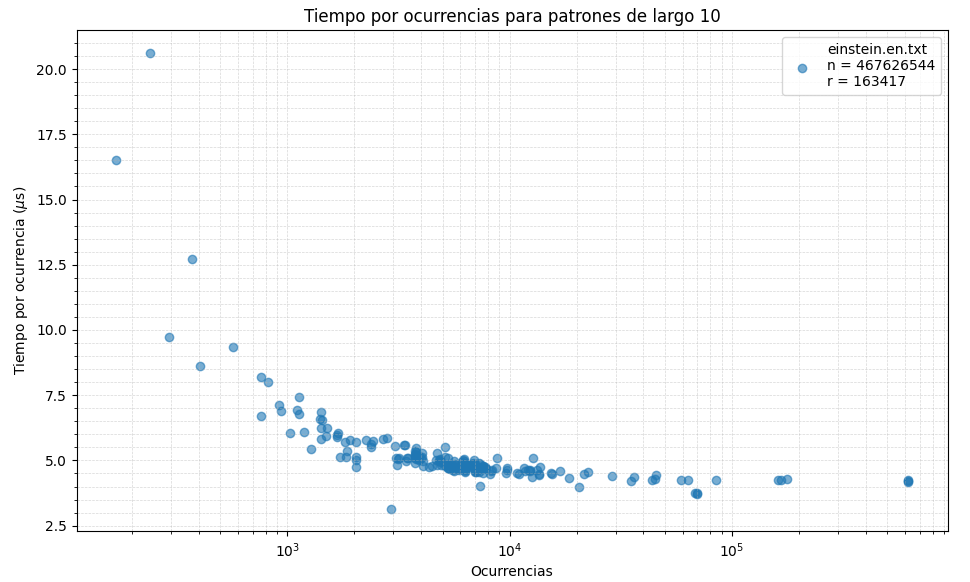
\includegraphics[width=1\textwidth]{imagenes/TIME_M10_EINSTEIN.png} 
    \label{fig:searcheinsteinm10}
\end{figure}

\section{Análisis comparativo con la solución lineal de búsqueda sin compresión}

El reporte de ocurrencia de patrones utilizando un algoritmo lineal en un texto sin comprimir tiene un tiempo de búsqueda en el peor caso de $\mathcal{O}(n m)$, con \textit{n} el largo del texto y \textit{m} el largo del patrón. En un texto real sin embargo, el tiempo es más cercano a $\mathcal{O}(n)$, pues la gran mayoría de las comparaciones terminan en el primer símbolo, es decir, el tiempo es relativamente independiente al largo del patrón.


\begin{table}[h!]
\centering
\begin{tabular}{|l|l|c|c|c|c|c|}
\hline
\textbf{n} & \textbf{r} & \textbf{m} & \textbf{occ} & \textbf{t(ms) estructura} & t(ms) lineal & t(ms) teórico \\ \hline
111299 & 26149 & 5 & 14 & \textbf{4.34} & 10.85 & 10.08 \\
111299 & 26149 & 10 & 1 & \textbf{4.36} & 10.76 & 10.17 \\
111299 & 26149 & 20 & 1 & \textbf{5.41} & 15.76 & 10.49 \\
111299 & 26149 & 30 & 1 & \textbf{6.14} & 15.74 & 10.98 \\
111299 & 26149 & 40 & 1 & \textbf{7.11} & 15.77 & 11.61 \\
111299 & 26149 & 50 & 1 & \textbf{7.85} & 15.88 & 12.41 \\
111299 & 26149 & 70 & 1 & \textbf{9.81} & 16.16 & 14.46 \\
111299 & 26149 & 100 & 1 & \textbf{11.72 }& 15.72 & 18.72 \\ \hline
290801 & 54170 & 5 & 93 & \textbf{7.88} & 28.77 & 10.17 \\
290801 & 54170 & 10 & 3 &\textbf{ 6.37 }& 28.68 & 10.20 \\
290801 & 54170 & 20 & 1 & \textbf{7.18} & 42.79 & 10.56 \\
290801 & 54170 & 30 & 1 & \textbf{8.15 }& 41.55 & 11.10 \\
290801 & 54170 & 40 & 1 & \textbf{9.24} & 42.41 & 11.81 \\
290801 & 54170 & 50 & 1 & \textbf{10.25} & 42.17 & 12.70 \\
290801 & 54170 & 70 & 1 & \textbf{12.41} & 41.76 & 14.98 \\
290801 & 54170 & 100 & 1 & \textbf{15.33} & 41.75 & 19.71 \\ \hline
704731 & 119734 & 5 & 640 & \textbf{21.11 }& 69.06 & 10.79 \\
704731 & 119734 & 10 & 216 & \textbf{12.15 }& 68.66 & 10.46 \\
704731 & 119734 & 20 & 75 & \textbf{10.71 }& 99.65 & 10.72 \\
704731 & 119734 & 30 & 1 & \textbf{ 9.41} & 99.67 & 11.24 \\
704731 & 119734 & 40 & 1 & \textbf{10.68} & 99.75 & 12.04 \\
704731 & 119734 & 50 & 1 & \textbf{11.78} & 99.69 & 13.02 \\
704731 & 119734 & 70 & 1 & \textbf{13.63} & 99.64 & 15.56 \\
704731 & 119734 & 100 & 1 & \textbf{16.94} & 99.26 & 20.80 \\ \hline
1224377 & 191364 & 5 & 329 & \textbf{17.24 }& 118.98 & 10.48 \\
1224377 & 191364 & 10 & 10 & \textbf{9.06} & 118.91 & 10.25 \\
1224377 & 191364 & 20 & 1 & \textbf{9.48} & 172.84 & 10.69 \\
1224377 & 191364 & 30 & 1 & \textbf{10.55} & 172.58 & 11.33 \\
1224377 & 191364 & 40 & 1 & \textbf{11.90} & 173.20 & 12.18 \\
1224377 & 191364 & 50 & 1 & \textbf{13.23} & 173.08 & 13.22 \\
1224377 & 191364 & 70 & 1 & \textbf{16.16} & 172.97 & 15.92 \\
1224377 & 191364 & 100 & 1 & \textbf{19.24} & 172.31 & 21.47 \\ \hline
2205984 & 333238 & 5 & 409 & \textbf{31.03} & 221.59 & 10.61 \\
2205984 & 333238 & 10 & 11 & \textbf{10.39} & 222.08 & 10.28 \\
2205984 & 333238 & 20 & 1 & \textbf{11.35} & 327.83 & 10.74 \\
2205984 & 333238 & 30 & 1 & \textbf{11.98 }& 320.78 & 11.43 \\
2205984 & 333238 & 40 & 1 & \textbf{13.65 }& 323.65 & 12.34 \\
2205984 & 333238 & 50 & 1 & \textbf{14.92} & 323.42 & 13.46 \\
2205984 & 333238 & 70 & 1 & \textbf{17.48} & 317.41 & 16.34 \\
2205984 & 333238 & 100 & 1 & \textbf{22.68} & 326.57 & 22.27 \\ \hline

\end{tabular}
\caption{Tiempos de búsqueda en textos reales de largo \textit{n} de patrones aleatorios de largo \textit{m}, con \textit{occ} ocurrencias en promedio y con \textit{r} la cantidad de reglas}
\label{tab:runtimes}
\end{table}

El costo temporal teórico de la estructura en reportar $occ$ ocurrencias, considerando $r$ como el número de reglas al comprimir el texto por gramática es:
\[
\mathcal{O}( (m + \log{n}) m \log{r} \log{\log{r}} + \textit{occ} \log{n} \log{\log{r}}  )
\]
Para que lo anterior sea menor al tiempo de búsqueda lineal, con un patrón de largo $m < \log {n}$ se debe cumplir que:
\[occ = o ( \frac{n}{ \log n \log \log r} ) \]

Los valores de \textit{occ} y \textit{r} serán pequeños si el texto es repetitivo y las ocurrencias del patrón de búsqueda son pocas. Este es el caso para textos reales como se aprecia en la tabla \ref{tab:runtimes}. Con largos de patrones suficientemente largos, las ocurrencias en textos reales tienden a ser únicas. La naturaleza de los textos reales hace que la "densidad" de repetitividad sea relativamente constante, y por lo tanto, la cantidad de ocurrencias de patrones crece más lento que el largo del texto. Esto implica que el algoritmo termina venciendo con más holgura a la búsqueda lineal mientras más largo sea el texto, al menos en el contexto de textos reales como lo son las novelas, los ensayos, \textit{etc}.

Con \textit{r} pequeño la grilla es pequeña y por lo tanto las búsquedas de rango son más cortas, además el árbol sintáctico es más pequeño y por lo tanto las búsquedas de ocurrencias hasta la raíz son más cortas. Con \textit{occ} pequeño la cantidad de búsquedas de ocurrencias son menores. Las ocurrencias \textit{occ} suelen ser proporcionales, tomando patrones aleatorios de un largo fijo, a qué tan repetitivo es el texto, es decir, en general, $occ \propto r ^{-1}$.

Para ejemplificar lo anterior, considere el siguiente texto $T$: 

\verb|"aaaaaaaaaabaaaaaaaaaab...aaaaaaaaaab\n..."|

Esto es, un texto de muchas líneas donde cada línea corresponde a la repetición de un patrón de cierta cantidad de \textit{a} seguidas de una \textit{b}. El texto es muy repetitivo, como se aprecia en la tabla \ref{tab:runtimes2} por la pequeña cantidad de reglas, y si se buscan patrones de la forma $a^{i}b$\verb|\n| que son los más raros, el buscador de la estructura es más rápido que la búsqueda lineal:

\begin{table}[h!]
\centering
\begin{tabular}{|l|l|c|c|c|c|c|}
\hline
\textbf{n} & \textbf{r} & \textbf{m} & \textbf{occ} & \textbf{t(ms) estructura} & t(ms) lineal & t(ms) teórico \\ \hline
69120 & 22 & 5 & 720 & 1.89 & 6.80 & 10.31 \\
69120 & 22 & 10 & 720 & 2.59 & 6.85 & 10.32 \\
69120 & 22 & 20 & 720 & 3.73 & 10.12 & 10.37 \\
69120 & 22 & 30 & 720 & 3.65 & 9.97 & 10.44 \\
69120 & 22 & 40 & 720 & 3.45 & 9.85 & 10.54 \\
69120 & 22 & 50 & 720 & 4.90 & 9.83 & 10.65 \\
69120 & 22 & 70 & 720 & 6.25 & 9.91 & 10.96 \\  \hline

\end{tabular}
\caption{Tiempos de búsqueda en texto repetitivo con \textit{n} el largo del texto original, \textit{r} la cantidad de reglas, \textit{m} el largo del patrón. }
\label{tab:runtimes2}
\end{table}

Considérese un ejemplo más realista. Se tiene una secuencia de ADN como un texto donde el alfabeto es $A, T, G, C$. Estas secuencias son sumamente largas, y buscar una cadena específica en esta usando una búsqueda lineal puede ser muy lento, en especial si se requiere repetir el proceso varias veces con distintos patrones de pocas ocurrencias. En este caso, la estructura tiene un tiempo de búsqueda más corto que la búsqueda lineal, como se aprecia en la tabla \ref{tab:runtimes3}.

\begin{table}[h!]
\centering
\begin{tabular}{|l|l|c|c|c|c|c|}
\hline
\textbf{n} & \textbf{r} & \textbf{m} & \textbf{occ} & \textbf{t(ms) estructura} & t(ms) lineal & t(ms) teórico \\ \hline  
1000000 & 182668 & 5 & 975 & 83.17 & 98.23 & 11.21 \\
1000000 & 182668 & 10 & 2 & 10.49 & 98.78 & 10.24 \\
1000000 & 182668 & 20 & 1 & 9.79 & 142.39 & 10.68 \\
1000000 & 182668 & 30 & 1 & 11.17 & 142.58 & 11.32 \\
1000000 & 182668 & 40 & 1 & 12.77 & 141.67 & 12.16 \\
1000000 & 182668 & 50 & 1 & 14.05 & 141.11 & 13.19 \\
1000000 & 182668 & 70 & 1 & 16.73 & 140.73 & 15.87 \\
1000000 & 182668 & 100 & 1 & 20.58 & 140.75 & 21.39 \\ \hline
\end{tabular}
\caption{Tiempos de búsqueda en secuencia de ADN de largo 100.000, \textit{occ} es la cantidad de ocurrencias del patrón}
\label{tab:runtimes3}
\end{table}




%\lambda + \lambda \log{r} + r \log{r}    +  2r \log r +       o(r \log r) +       2r \log \sigma
% 16  + 16log16112 + 16112log16112+  2*16112 log 16112 + 16112 log 16112 + 2*16112 log 16112
% 16  + 16 * 14 + 16112*14 +  16112*32 + 16112*14 + 16112*32

\section{Análisis comparativo con índice comprimido basado en gramática}

El índice comprimido basado en gramática\cite{claude2020} es una estructura de datos que permite buscar patrones en un texto comprimido por gramática. La tabla \ref{tab:runtimes4} muestra los tiempos de búsqueda de patrones aleatorios en textos reales con la estructura propuesta en este trabajo y con la estructura del índice comprimido basado en gramática.


\begin{table}[h!]
\centering
\begin{tabular}{|l|l|c|c|c|c|c|}
\hline
\textbf{set} & \textbf{tamaño} & \textbf{m} & \textbf{occ} & \textbf{t(ms) estructura} & t(ms) índice \\ \hline  

\hline
\end{tabular}
\caption{Tiempos de búsqueda para patrones aleatorios de largo \textit{m}, con \textit{occ} ocurrencias}
\label{tab:runtimes4}
\end{table}